% Options for packages loaded elsewhere
\PassOptionsToPackage{unicode}{hyperref}
\PassOptionsToPackage{hyphens}{url}
\PassOptionsToPackage{dvipsnames,svgnames,x11names}{xcolor}
%
\documentclass[
  11pt,
]{article}
\usepackage{amsmath,amssymb}
\usepackage{iftex}
\ifPDFTeX
  \usepackage[T1]{fontenc}
  \usepackage[utf8]{inputenc}
  \usepackage{textcomp} % provide euro and other symbols
\else % if luatex or xetex
  \usepackage{unicode-math} % this also loads fontspec
  \defaultfontfeatures{Scale=MatchLowercase}
  \defaultfontfeatures[\rmfamily]{Ligatures=TeX,Scale=1}
\fi
\usepackage{lmodern}
\ifPDFTeX\else
  % xetex/luatex font selection
\fi
% Use upquote if available, for straight quotes in verbatim environments
\IfFileExists{upquote.sty}{\usepackage{upquote}}{}
\IfFileExists{microtype.sty}{% use microtype if available
  \usepackage[]{microtype}
  \UseMicrotypeSet[protrusion]{basicmath} % disable protrusion for tt fonts
}{}
\makeatletter
\@ifundefined{KOMAClassName}{% if non-KOMA class
  \IfFileExists{parskip.sty}{%
    \usepackage{parskip}
  }{% else
    \setlength{\parindent}{0pt}
    \setlength{\parskip}{6pt plus 2pt minus 1pt}}
}{% if KOMA class
  \KOMAoptions{parskip=half}}
\makeatother
\usepackage{xcolor}
\usepackage[margin=1in]{geometry}
\usepackage{color}
\usepackage{fancyvrb}
\newcommand{\VerbBar}{|}
\newcommand{\VERB}{\Verb[commandchars=\\\{\}]}
\DefineVerbatimEnvironment{Highlighting}{Verbatim}{commandchars=\\\{\}}
% Add ',fontsize=\small' for more characters per line
\newenvironment{Shaded}{}{}
\newcommand{\AlertTok}[1]{\textcolor[rgb]{1.00,0.00,0.00}{\textbf{#1}}}
\newcommand{\AnnotationTok}[1]{\textcolor[rgb]{0.38,0.63,0.69}{\textbf{\textit{#1}}}}
\newcommand{\AttributeTok}[1]{\textcolor[rgb]{0.49,0.56,0.16}{#1}}
\newcommand{\BaseNTok}[1]{\textcolor[rgb]{0.25,0.63,0.44}{#1}}
\newcommand{\BuiltInTok}[1]{\textcolor[rgb]{0.00,0.50,0.00}{#1}}
\newcommand{\CharTok}[1]{\textcolor[rgb]{0.25,0.44,0.63}{#1}}
\newcommand{\CommentTok}[1]{\textcolor[rgb]{0.38,0.63,0.69}{\textit{#1}}}
\newcommand{\CommentVarTok}[1]{\textcolor[rgb]{0.38,0.63,0.69}{\textbf{\textit{#1}}}}
\newcommand{\ConstantTok}[1]{\textcolor[rgb]{0.53,0.00,0.00}{#1}}
\newcommand{\ControlFlowTok}[1]{\textcolor[rgb]{0.00,0.44,0.13}{\textbf{#1}}}
\newcommand{\DataTypeTok}[1]{\textcolor[rgb]{0.56,0.13,0.00}{#1}}
\newcommand{\DecValTok}[1]{\textcolor[rgb]{0.25,0.63,0.44}{#1}}
\newcommand{\DocumentationTok}[1]{\textcolor[rgb]{0.73,0.13,0.13}{\textit{#1}}}
\newcommand{\ErrorTok}[1]{\textcolor[rgb]{1.00,0.00,0.00}{\textbf{#1}}}
\newcommand{\ExtensionTok}[1]{#1}
\newcommand{\FloatTok}[1]{\textcolor[rgb]{0.25,0.63,0.44}{#1}}
\newcommand{\FunctionTok}[1]{\textcolor[rgb]{0.02,0.16,0.49}{#1}}
\newcommand{\ImportTok}[1]{\textcolor[rgb]{0.00,0.50,0.00}{\textbf{#1}}}
\newcommand{\InformationTok}[1]{\textcolor[rgb]{0.38,0.63,0.69}{\textbf{\textit{#1}}}}
\newcommand{\KeywordTok}[1]{\textcolor[rgb]{0.00,0.44,0.13}{\textbf{#1}}}
\newcommand{\NormalTok}[1]{#1}
\newcommand{\OperatorTok}[1]{\textcolor[rgb]{0.40,0.40,0.40}{#1}}
\newcommand{\OtherTok}[1]{\textcolor[rgb]{0.00,0.44,0.13}{#1}}
\newcommand{\PreprocessorTok}[1]{\textcolor[rgb]{0.74,0.48,0.00}{#1}}
\newcommand{\RegionMarkerTok}[1]{#1}
\newcommand{\SpecialCharTok}[1]{\textcolor[rgb]{0.25,0.44,0.63}{#1}}
\newcommand{\SpecialStringTok}[1]{\textcolor[rgb]{0.73,0.40,0.53}{#1}}
\newcommand{\StringTok}[1]{\textcolor[rgb]{0.25,0.44,0.63}{#1}}
\newcommand{\VariableTok}[1]{\textcolor[rgb]{0.10,0.09,0.49}{#1}}
\newcommand{\VerbatimStringTok}[1]{\textcolor[rgb]{0.25,0.44,0.63}{#1}}
\newcommand{\WarningTok}[1]{\textcolor[rgb]{0.38,0.63,0.69}{\textbf{\textit{#1}}}}
\usepackage{longtable,booktabs,array}
\usepackage{calc} % for calculating minipage widths
% Correct order of tables after \paragraph or \subparagraph
\usepackage{etoolbox}
\makeatletter
\patchcmd\longtable{\par}{\if@noskipsec\mbox{}\fi\par}{}{}
\makeatother
% Allow footnotes in longtable head/foot
\IfFileExists{footnotehyper.sty}{\usepackage{footnotehyper}}{\usepackage{footnote}}
\makesavenoteenv{longtable}
\usepackage{graphicx}
\makeatletter
\def\maxwidth{\ifdim\Gin@nat@width>\linewidth\linewidth\else\Gin@nat@width\fi}
\def\maxheight{\ifdim\Gin@nat@height>\textheight\textheight\else\Gin@nat@height\fi}
\makeatother
% Scale images if necessary, so that they will not overflow the page
% margins by default, and it is still possible to overwrite the defaults
% using explicit options in \includegraphics[width, height, ...]{}
\setkeys{Gin}{width=\maxwidth,height=\maxheight,keepaspectratio}
% Set default figure placement to htbp
\makeatletter
\def\fps@figure{htbp}
\makeatother
\setlength{\emergencystretch}{3em} % prevent overfull lines
\providecommand{\tightlist}{%
  \setlength{\itemsep}{0pt}\setlength{\parskip}{0pt}}
\setcounter{secnumdepth}{-\maxdimen} % remove section numbering
\usepackage{amsmath,amssymb,mathpazo}
\newcommand{\llbracket}{\mathopen{[\![}}
\newcommand{\rrbracket}{\mathclose{]\!]}}
\usepackage{microtype}
\usepackage{float,etoolbox}
\floatplacement{figure}{H}
\AtBeginEnvironment{longtable}{\small\setlength{\tabcolsep}{4pt}}
\setlength{\emergencystretch}{3em}
\ifLuaTeX
  \usepackage{selnolig}  % disable illegal ligatures
\fi
\IfFileExists{bookmark.sty}{\usepackage{bookmark}}{\usepackage{hyperref}}
\IfFileExists{xurl.sty}{\usepackage{xurl}}{} % add URL line breaks if available
\urlstyle{same}
\hypersetup{
  pdftitle={Caprice: Higher-Categorical Semantics of Capture-Aware Partial Evaluation and JIT Matching},
  pdfauthor={Anonymous author},
  colorlinks=true,
  linkcolor={blue},
  filecolor={Maroon},
  citecolor={Blue},
  urlcolor={blue},
  pdfcreator={LaTeX via pandoc}}

\title{Caprice: Higher-Categorical Semantics of Capture-Aware Partial
Evaluation and JIT Matching}
\author{Anonymous author}
\date{October 24, 2026}

\begin{document}
\maketitle

\hypertarget{abstract}{%
\subsection{Abstract}\label{abstract}}

We present a byte-oriented pattern language combining named captures,
backreferences, literal interpolation, and fully applied typed lambdas
over a small total string language. Its semantics distinguishes
acceptance, capture observations, ordered matching witnesses, and
resource exhaustion. Matching is modeled by ordered state
transformations and witness correspondences in a presheaf infinity-topos
of static-information worlds. A localization of certified rewrites
records optimization paths without identifying observational equivalence
with execution cost. We prove expression specialization, ordered-match
preservation, and a conditional simulation theorem for native
control-flow compilation. A Lean 4 kernel model checks specialization
and strictness results. A Rust implementation includes a parser,
backtracking VM, partial evaluator, and Cranelift JIT. Reproducible
experiments compare three implementation modes with PCRE2, PCRE2 JIT,
Rust regex, and CPython re. Across 11 synthetic workloads,
specialization improves median matching latency by 1.30 to 22.02 times
over the raw VM (2.89 times geometric mean), while the helper-based JIT
is slower than the specialized VM on every measured median. These
results establish a working research artifact and identify remaining
engineering costs; they do not establish universal superiority over
existing engines.

\textbf{Keywords:} backreferences; partial evaluation; typed
interpolation; capture semantics; presheaf infinity-topos; native
compilation; reproducible benchmarking.

\hypertarget{problem-and-contribution}{%
\subsection{1. Problem and
contribution}\label{problem-and-contribution}}

A captured string is useful both as data to be compared with a later
substring and as an argument to an acceptance predicate. For example, an
identifier may be followed by its ASCII uppercase rendering, while a
typed predicate restricts the identifier's length. A general-purpose
host-language callback can express this behavior, but leaves the
embedded language, effects, and specialization boundary unspecified.
Caprice instead provides a small explicit calculus and a Rust
implementation.

The contribution is a combination of four artifacts: a precise pattern
language; a higher-categorical organization of its semantics and
certified transformations; a tested partial evaluator and native
control-flow compiler; and measured comparisons with existing engines.
The paper does not claim that backreferences, callouts, partial
evaluation, or regex JIT compilation are new. PCRE2 already offers
callouts and JIT {[}3,4{]}; the distinction here is the explicitly
typed, total expression fragment and the treatment of optimization
correctness, witness structure, and costs in one specification.

Backreferences extend expressive power beyond regular languages. Their
general matching problem is NP-complete when the pattern is part of the
input; restricted classes admit better algorithms {[}2{]}. Specializing
a pattern does not remove that general boundary. Rust regex deliberately
omits backreferences and documents an \(O(mn)\) worst-case search bound,
where \(m\) measures the regex and \(n\) the subject {[}5{]}. We
therefore mark unsupported comparisons, rather than assigning
regular-only engines incorrect substitutes for backreference matching.

\hypertarget{surface-language-and-types}{%
\subsection{2. Surface language and
types}\label{surface-language-and-types}}

Let \(\Sigma=\{0,\ldots,255\}\) and \(\mathrm{Str}=\Sigma^*\). A match
consumes the entire input. The public syntax supports literal bytes,
classes, dot excluding LF, concatenation, left-priority alternation,
named captures, named backreferences, greedy or lazy bounded/unbounded
repetition, and absolute start/end assertions. Plain capturing
parentheses are deliberately rejected; use
\texttt{(?\textless{}name\textgreater{}...)} or \texttt{(?:...)}.
Numeric backreferences, lookaround, Unicode character semantics,
recursive patterns, search offsets, and replacement APIs are outside
version 0.1.

The two extensions are:

\begin{Shaded}
\begin{Highlighting}[]
\NormalTok{$\{e\}       evaluate e : Str and consume exactly its resulting bytes}
\NormalTok{(?\{e\})     evaluate e : Bool; retain this branch exactly when true}
\end{Highlighting}
\end{Shaded}

Interpolation is literal matching, never reparsing the result as regex
source. For instance, the static value \texttt{.*} consumes a dot and an
asterisk. Expressions use parenthesized operator application; string
tokens use JSON string syntax. There is no implicit coercion, implicit
capture lookup, host \texttt{eval}, recursion, I/O, or mutation. The
core grammar is:

\begin{Shaded}
\begin{Highlighting}[]
\NormalTok{T ::= Str | Nat | Bool}
\NormalTok{e ::= "JSON string" | unsigned{-}integer | true | false | x}
\NormalTok{    | (cap name) | (param name) | (op e ... e)}
\NormalTok{    | (call (lambda (x T) e) e)}
\end{Highlighting}
\end{Shaded}

Lambdas are first-order and syntactically fully applied. They can nest
and shadow variables, but cannot be stored or passed as function values.
Static parameters have type \texttt{Str}; every referenced parameter
must be supplied before compilation. A capture name must already have
been declared, but need not have participated in the current branch. The
operators are:

\begin{longtable}[]{@{}
  >{\raggedright\arraybackslash}p{(\columnwidth - 2\tabcolsep) * \real{0.5000}}
  >{\raggedright\arraybackslash}p{(\columnwidth - 2\tabcolsep) * \real{0.5000}}@{}}
\toprule\noalign{}
\begin{minipage}[b]{\linewidth}\raggedright
Operators
\end{minipage} & \begin{minipage}[b]{\linewidth}\raggedright
Signature and meaning
\end{minipage} \\
\midrule\noalign{}
\endhead
\bottomrule\noalign{}
\endlastfoot
\texttt{lower}, \texttt{upper}, \texttt{trim} &
\(\mathrm{Str}\to\mathrm{Str}\); ASCII case conversion / ASCII
whitespace trimming \\
\texttt{concat} & \(\mathrm{Str}^2\to\mathrm{Str}\); concatenation \\
\texttt{slice} & \(\mathrm{Str}\times\mathrm{Nat}^2\to\mathrm{Str}\);
half-open byte slice, endpoints clamped \\
\texttt{len} & \(\mathrm{Str}\to\mathrm{Nat}\); byte length \\
\texttt{eq} & \(T\times T\to\mathrm{Bool}\) for a common base type
\(T\) \\
\texttt{contains}, \texttt{starts}, \texttt{ends} &
\(\mathrm{Str}^2\to\mathrm{Bool}\); byte predicates \\
\texttt{lt}, \texttt{le} & \(\mathrm{Nat}^2\to\mathrm{Bool}\) \\
\texttt{and}, \texttt{or}, \texttt{not} & Boolean operators; operands
evaluated strictly \\
\end{longtable}

Here \texttt{slice(s,a,b)} means \(s[a':b']\), with \(a'=\min(a,|s|)\)
and \(b'=\max(a',\min(b,|s|))\). An empty substring is contained in
every string. The implementation parses natural literals as
\texttt{usize}; its lengths are machine-representable. The abstract
model uses natural numbers. It contains no arithmetic operation that
could overflow.

More precisely, \texttt{trim} removes bytes 9, 10, 12, 13, and 32,
following Rust's ASCII-whitespace predicate; the pattern shorthand
\texttt{\textbackslash{}s} additionally includes byte 11. Case
conversion changes ASCII letters only. Arbitrary other bytes are
preserved.

For example, the following is one pattern, written on separate lines
only for readability (the parser does not ignore whitespace):

\begin{Shaded}
\begin{Highlighting}[]
\NormalTok{(?\textless{}x\textgreater{}[A{-}Za{-}z]+):$\{(upper (cap x))\}}
\NormalTok{(?\{(call (lambda (s Str) (le (len s) 5)) (cap x))\})}
\end{Highlighting}
\end{Shaded}

It accepts \texttt{Abc:ABC}, rejects \texttt{Abc:abc}, and rejects an
identifier longer than five bytes.

\textbf{Definition 2.1 (partial capture environment).} For input \(w\)
of length \(n\) and a finite set \(K\) of capture names, let
\(\mathrm{Span}_n=\{(a,b):0\leq a\leq b\leq n\}\) and
\(\gamma:K\to\mathrm{Span}_n+\{\bot\}\). A participating empty capture
is \((a,a)\); it is distinct from \(\bot\). Reading an unset or
currently open capture yields \texttt{None}.

\textbf{Definition 2.2 (strict expression evaluation).} A well-typed
expression has interpretation

\[
\mathopen{[\![}e:T\mathclose{]\!]}_{w,\gamma,\rho,\eta}\in\operatorname{Option}(\mathopen{[\![}T\mathclose{]\!]}),
\]

where \(\rho\) supplies static parameters and \(\eta\) supplies
lambda-bound variables. Constants evaluate to \texttt{Some}; a defined
capture evaluates to \(w[a:b]\). Primitive operators lift their total
functions by strict left-to-right \texttt{Option} sequencing. Lambda
application first evaluates its argument and, if defined, evaluates the
body in the extended lexical environment. An undefined argument is not
discarded even when its variable is unused. A guard accepts only
\texttt{Some(true)}; interpolation consumes only a defined string.

\textbf{Lemma 2.3 (termination and type preservation).} Every well-typed
expression terminates with either a value of its specified type or
\texttt{None}.

\emph{Proof.} The source AST is finite, primitive functions terminate on
finite byte strings, and application evaluates two structurally nested
expressions without recursion. Induction on the typed AST gives the
claim; lexical environments provide values at the declared types. This
lemma concerns mathematical evaluation, not unlimited physical memory.
\(\square\)

\hypertarget{ordered-matching-and-backtracking}{%
\subsection{3. Ordered matching and
backtracking}\label{ordered-matching-and-backtracking}}

For fixed \(w\), a state is \(s=(i,\gamma)\) with \(0\leq i\leq |w|\).
Interpret a pattern as an ordered list of successor states,
\(R_p:S_w\to\operatorname{List}(S_w)\). Empty matching is the singleton
identity and failure is the empty list. Alternation concatenates lists
in source order; sequence uses list bind:

\[
R_{p;q}(s)=\operatorname{concat}_{t\in R_p(s)}R_q(t),\qquad
R_{p\mid q}(s)=R_p(s)\mathbin{+\!+}R_q(s).
\]

A literal consumes its own prefix or fails. A backreference consumes
\(w[a:b]\) when its capture is defined. Capture \(k\) records the
starting position, clears the old binding while evaluating its body, and
writes the resulting span on each successful branch. Other capture
bindings are retained. Each alternative restores its saved state; failed
branches cannot leak capture updates.

Repetition follows the recursive prioritized choice used by the VM, not
an unordered union over lengths. A greedy optional continuation tries
the body and another iteration before the empty exit; lazy repetition
tries that exit first. Bounded repetition decreases its remaining count.
Unbounded repetition is admitted only when a conservative nullability
analysis proves the body consumes a byte on every success. In
particular, a backreference or dynamic interpolation is conservatively
treated as possibly empty even if more detailed analysis could prove
otherwise.

\textbf{Definition 3.1 (observations).} Starting from position zero and
all captures unset, filter the successor list to states at position
\(|w|\). Write \(\mathcal O(p,\rho,w)\) for the resulting ordered list
of capture environments, retaining multiplicity. Boolean acceptance
tests nonemptiness; the implementation returns the first environment.
Complete ordered observations are stronger than either
returned-first-capture equivalence or Boolean language equivalence.

\textbf{Proposition 3.2 (finite reference search).} Every accepted
source pattern has a finite search tree on each finite input.

\emph{Proof.} Bounded repetitions expand into finite control flow. Every
cycle of an unbounded repetition contains a successful consuming body; a
successful path can traverse such cycles only finitely often before
exhausting the input. The remaining acyclic paths have finite branching.
False predicates and unset reads terminate individual branches.
\(\square\)

\textbf{Counterexample 3.3 (postfiltering the first match is unsound).}
Consider

\begin{Shaded}
\begin{Highlighting}[]
\NormalTok{(?\textless{}x\textgreater{}a|aa)a?(?\{(eq (cap x) "aa")\})}
\end{Highlighting}
\end{Shaded}

on \texttt{aa}. The first ordinary full match captures \texttt{a}; its
guard fails. Backtracking finds the capture \texttt{aa}, whose guard
succeeds. Calling an old engine once and postfiltering its first match
would reject. Baseline postprocessors in Section 8 are therefore used
only on patterns whose full-match captures are unique. PCRE2 callouts
could support a broader internal-predicate comparison {[}4{]}, but such
a baseline is not implemented here.

\hypertarget{higher-categorical-organization}{%
\subsection{4. Higher-categorical
organization}\label{higher-categorical-organization}}

Fix a finite static-parameter signature \(M\). A \emph{world} \(\sigma\)
assigns byte strings to a subset of \(M\). Define a small category \(W\)
with a unique arrow \(\tau\to\sigma\) when \(\tau\) extends \(\sigma\).
Let \(\Omega_\sigma\) be the set of total assignments extending
\(\sigma\). The inclusion \(\Omega_\tau\hookrightarrow\Omega_\sigma\)
induces restriction of behavior functions. Consequently

\[
\mathcal E=\operatorname{Fun}(W^{\mathrm{op}},\mathcal S),\qquad
B(\sigma)=\operatorname{Set}\bigl(\Omega_\sigma\times\Sigma^*,
\operatorname{List}(\mathrm{CapResult})\bigr)
\]

define a presheaf infinity-topos and a discrete-valued behavior object
in it. Capture results include their input-compatible spans. No extra
Grothendieck topology or descent assumption is imposed. The assertion
that \(\mathcal E\) is an infinity-topos is the standard presheaf
construction {[}6{]}, not a claim that a regex automaton or a
program-localization category is itself a topos.

\textbf{Definition 4.1 (matching witnesses).} Let \(D_p\) be the family
of finite derivations of successful transitions. With source and target
maps it determines a correspondence

\[ S\xleftarrow{\;s\;}D_p\xrightarrow{\;t\;}S. \]

Here the subject and total parameters are carried unchanged in the state
family. All these objects can be regarded as presheaves over \(W\) by
restricting the allowed completions. Concatenation composes
correspondences through a homotopy pullback; alternatives use tagged
coproducts. In the present implementation the fibers are sets, so these
homotopy pullbacks reduce to ordinary pullbacks. The higher formulation
permits structured witness spaces without changing the base
construction. Correspondence calculi and higher categories of spans
provide the relevant general framework {[}7{]}.

The hom infinity-category \(\mathcal E_{/X\times Y}\), with pullback
composition, also gives a calculus of spans with maps of spans as
refinements. A refinement need not be an equivalence of witness objects.
Coherent associativity comes from the universal property of pullbacks.
Execution priority remains additional list/branch-order data; plain
correspondences do not encode which result a greedy engine returns
first.

\textbf{Proposition 4.2 (levels of observation).} The image of
\(D_p\to S\times S\) is the successful transition relation; its fibers
are the \((-1)\)-truncations of witness fibers. Further existential
projection to complete input matches gives Boolean acceptance. Neither
construction in general recovers ordered capture results.

\emph{Proof.} Image factorization in an infinity-topos is fiberwise
propositional truncation. An inhabited derivation fiber records
existence of the corresponding transition. Existential projection
forgets the selected capture state as well. Reversing the alternatives
in \texttt{(?\textless{}x\textgreater{}a\textbar{}aa)a?} leaves
acceptance of \texttt{aa} unchanged but changes the first capture,
establishing the final assertion. \(\square\)

For each world, let \(\mathcal R_\sigma\) be the small category
presented by finite programs, selected certified rewrite steps, and
declared equations between rewrite paths. Certificates assert equality
in \(B(\sigma)\). Restriction of a certificate to fewer completions
defines its image at an extending world. Let

\[ C(\sigma)=\mathcal R_\sigma[\operatorname{Mor}(\mathcal R_\sigma)^{-1}] \]

denote its infinity-groupoid completion, retaining the nerve's homotopy
information rather than replacing it by a set of connected components.
Functorial localization makes \(C\) an object of \(\mathcal E\). Sound
rewrite generators induce a natural observation map
\(\operatorname{obs}:C\to B\): the map factors through localization
because every generating rewrite becomes equality of behaviors. Declared
coherence equations must themselves be justified; they are not inferred
merely from matching test outputs. For example, disjoint
constant-folding rewrites commute because they replace different AST
subtrees.

\textbf{Definition 4.3 (implementation fiber).} For the behavior section
\(b_p:1\to B\) of a program, define

\[ \mathcal F_p=1\mathbin{\times}_{B} C. \]

Points describe compatible implementations; paths describe certified
rewrite equivalences, and higher paths describe the coherences retained
by the chosen presentation. No nontrivial higher homotopy group is
asserted or computed for this prototype. The construction specifies
where such information belongs. It distinguishes a proof-bearing
optimization history from the mere assertion that two programs accept
the same language.

\hypertarget{partial-evaluation-and-preservation}{%
\subsection{5. Partial evaluation and
preservation}\label{partial-evaluation-and-preservation}}

The implementation specializes against the pattern syntax and supplied
static parameters. It replaces parameter reads with literals, folds
closed primitive applications, beta-reduces fully applied lambdas with
static arguments, removes constant guards, changes constant
interpolation into literal matching, fuses adjacent literals, and
replaces class-only repeats with a scanner plus ordered backtracking
alternatives. Dynamic lambda arguments remain strict. Static folding is
capped at 1 MiB for an individual computed string; a larger expression
remains residual.

\textbf{Theorem 5.1 (expression specialization).} Let \(\rho\) extend
\(\sigma\). For every well-typed expression and capture environment,

\[ \mathopen{[\![}\operatorname{pe}_\sigma(e)\mathclose{]\!]}_{w,\gamma,\rho,\eta}
=\mathopen{[\![}e\mathclose{]\!]}_{w,\gamma,\rho,\eta}. \]

\emph{Proof.} Induct on the typed expression. Known parameter
replacement is sound because the completion agrees with \(\sigma\).
Closed primitive folding applies the same total function to the same
values. If the specialized lambda argument is a value, lexical value
substitution yields the body evaluation. Otherwise the residual
application retains argument evaluation before the body, including
\texttt{None}. The inductive hypotheses cover remaining subexpressions.
Refusing an oversized fold simply retains an expression whose recursive
specializations are sound. \(\square\)

The attached \texttt{formal/Specialization.lean} checks the analogous
theorem for an intrinsically typed kernel with arbitrary total
unary/binary primitives, captures, partially known parameters, and
strict fully applied lambdas represented by higher-order abstract
syntax. It also proves semantic agreement of successive specialization
stages and guard preservation. The checked artifact uses Lean 4.19.0
{[}12{]} with the standard logical axioms reported in its validation
log; it contains no \texttt{sorry} or added axiom. It does \textbf{not}
verify extraction to Rust, the parser, bounded allocation, the regex VM,
or Cranelift.

\textbf{Lemma 5.2 (strictness is essential).} In general,
\texttt{(call\ (lambda\ (x\ Str)\ true)\ (cap\ missing))} cannot
specialize to \texttt{true}.

\emph{Proof.} The former evaluates to \texttt{None} when the capture is
unset; the latter evaluates to \texttt{Some(true)}. This law is also
checked in Lean and tested in all three engine modes. \(\square\)

\textbf{Theorem 5.3 (ordered-match preservation).} In the
unbounded-resource semantics, specialization preserves
\(\mathcal O(p,\rho,w)\), hence both acceptance and the first returned
capture environment.

\emph{Proof.} Theorem 5.1 preserves each guard and interpolated literal.
Removing a true guard or combining successive literals removes
deterministic administrative steps and preserves ordered successors.
Class-repeat fusion enumerates exactly the same lengths in the same
priority order, and the fused body changes no capture. Sequence and
alternation preserve equality by list bind and concatenation. Bounded
repetition follows by induction on its bound; consuming unbounded
repetition follows by induction on remaining input length. These
arguments produce a correspondence of successful observations, without
requiring arbitrary optimization histories to have identical trace
presentations. \(\square\)

The compiler additionally moves an end-of-input assertion before a
contiguous trailing suffix of zero-width guards. Both tests leave the
state unchanged, so filtering by end position commutes with guard
filtering. The observation is full matching, making this transformation
sound even though it would require a different argument for substring
search. Control-flow targets are relocated to preserve entry into the
guard suffix. This optimization is included in the measured PE and JIT
modes.

\textbf{Proposition 5.4 (budgets are not preserved by PE).} Equal
unbounded observations do not imply equal outcomes under a fixed
operational budget.

\emph{Proof.} A raw sequence of \(k\) one-byte literal instructions can
require \(k\) dispatches, while its fused literal uses one. Choose a
dispatch budget between these values. One program may exhaust it while
the other matches. Hoisting an end assertion may likewise avoid an
expression allocation on a branch that cannot complete. \(\square\)

\hypertarget{rust-vm-and-native-control-flow-compiler}{%
\subsection{6. Rust VM and native control-flow
compiler}\label{rust-vm-and-native-control-flow-compiler}}

The parser produces a typed expression AST and pattern AST. Compilation
emits instructions for literals, classes, capture start/end,
backreferences, guards, interpolation, branching, jumps, assertions,
acceptance, and failure. A backtracking frame stores a program counter,
input position, and complete capture snapshot. Entering a capture
invalidates its previous value until its end instruction. Snapshot
restoration is the rollback invariant.

\texttt{raw} executes unspecialized bytecode. \texttt{pe} executes
specialized bytecode. \texttt{jit} compiles that same specialized
program to native code with Cranelift 0.125.3. Every instruction gets a
native control-flow block; successful edges are compiled directly, while
a dynamic backtracking target is selected through a compiled switch. The
generated code calls checked Rust helpers for instruction effects,
string operators, captures, and budgets. Thus this is a \textbf{native
control-flow JIT}, not a native compiler for each string operator, a
regex DFA generator, or a fully inlined tracing JIT. The runtime helper
still dispatches on the opcode. This deliberate implementation boundary
is important when interpreting performance.

\textbf{Theorem 6.1 (conditional JIT simulation).} Assume the native
compiler and C ABI correctly implement the generated control-flow graph,
the runtime helper implements the specified bytecode transition, and
code/environment lifetimes are valid. The VM and JIT on the same
residual program return the same capture result, failure, or budget
exhaustion.

\emph{Proof.} Relate a VM state at instruction \(j\) to a native
invocation at block \(j\) with the same Rust runtime record. Both call
the same instruction transition. Success follows the same statically
determined edge; failure invokes the same frame-pop operation and
reaches the corresponding block or terminal failure. Exhaustion returns
immediately in both. Acceptance requires the same input end position and
retains the same capture array. Induction on dispatches proves lockstep
simulation. The theorem is conditional: the artifact does not contain a
machine-checked proof of Cranelift, generated machine code, or Rust's
FFI implementation. \(\square\)

Default matching limits are one million dispatches, 100,000 pending
frames, and 1 MiB per expression string. Source size is capped at 8,192
bytes, capture count at 128, nesting at 128, repetition counts at 1,000,
and expanded programs at 32,768 instructions. These are safeguards, not
a proof of a fixed wall-clock bound or a global memory quota: one
primitive may scan many bytes, and snapshots may be large. Exhaustion is
a separate result, never silently converted to rejection. A production
service would additionally need explicit total memory accounting, time
cancellation, caching policies, and a hardened deployment boundary.

\hypertarget{correctness-evidence}{%
\subsection{7. Correctness evidence}\label{correctness-evidence}}

The final Rust release test run passes nine tests. An exhaustive suite
covers 19 shared patterns on all 1,093 strings of length at most six
over \texttt{ab-}: 20,767 pattern/input cases. It compares acceptance
and every capture span with PCRE2 and compares all three Caprice modes.
A second suite covers four extended patterns on all 3,906 strings of
length at most five over \texttt{abAB-}: 15,624 cases comparing the
three modes. These are 36,391 cases, not an exhaustive proof over all
patterns. Separate regressions cover lexical shadowing, unset/empty
captures, rollback, type errors, literal parameter injection, budget
outcomes, and correct bounded-repeat compilation.

Benchmark preflight separately validates every timed
engine/workload/input combination against explicit expected answers.
Each timed sample checks its aggregate accepted count. Rust formatting
and Clippy with warnings denied pass. Lean logs and dependency versions
are included. Exhaustive bounded tests, a small checked model, and
conditional mathematical proofs provide different kinds of evidence and
should not be conflated.

\hypertarget{experimental-protocol}{%
\subsection{8. Experimental protocol}\label{experimental-protocol}}

The measurements were produced in an x86-64 Linux container on an AMD
EPYC 9V74 host, pinned to logical CPU 0. The visible CPU frequency was
approximately 2.60 GHz; frequency and other host tenants were not
controlled. The build used Rust 1.99.1 with
\texttt{cargo\ build\ -\/-release\ -\/-locked}, default CPU targeting,
and no extra \texttt{RUSTFLAGS}. Baselines were PCRE2 10.42 without JIT,
PCRE2 10.42 with successful JIT compilation, Rust regex 1.12.2, and
CPython 3.12.14. Versions are the tested installations, not a claim to
use every engine's latest release. The primary compiler packages are
Cranelift 0.125.3; \texttt{Cargo.lock} records all transitive versions.

There are 11 deterministic synthetic workloads, each with 256 inputs and
half accepted. The corpus generator is included. Full byte matching,
ASCII transforms, no locale dependence, and absolute end semantics are
aligned. Both backreference workloads are omitted from Rust regex.
Static interpolation is compiled into the baseline regex. Three dynamic
workloads use a baseline regex plus a host predicate on uniquely
determined full-match captures: ASCII case equality, uppercase-pair
equality, or length at most 16. Their timings include the predicate.
This translation is justified only by uniqueness for these selected
workloads; Counterexample 3.3 prohibits treating it as a general
implementation of Caprice guards.

Each of three fresh process runs builds every engine/pattern seven times
for compilation timing, validates all inputs, performs warm-up passes,
and calibrates a batch toward 20 ms. Nine timed batches per job are
interleaved in deterministic shuffled order. Thus each table entry
aggregates 27 matching samples and 21 compile samples. The primary
statistic is the median per-input latency; raw samples and inclusive
interquartile ranges are supplied. CPython runs separately and includes
Python loop and call overhead, whereas the other timed loops are Rust.
Boolean queries use each engine's normal API: PCRE2 reuses its match
data, while Caprice allocates capture state per invocation. These API
differences are part of this implementation comparison, not a controlled
comparison of identical allocation strategies.

Compilation is excluded from warm matching and measured separately.
Cranelift function bytes and PCRE2 reported JIT bytes are recorded, but
are not equated with total memory usage. The experiments do not measure
production throughput, concurrent use, JIT cache eviction, energy, peak
resident memory by engine, Unicode workloads, Ruby/Onigmo, or large
real-world corpora. IQRs measure sample dispersion, not inferential
confidence.

\hypertarget{results-and-interpretation}{%
\subsection{9. Results and
interpretation}\label{results-and-interpretation}}

The following values are median \textbf{nanoseconds per full-match
decision}; lower is better. Host predicates are included where
applicable. A dash means unsupported.

\begin{longtable}[]{@{}
  >{\raggedright\arraybackslash}p{(\columnwidth - 14\tabcolsep) * \real{0.2727}}
  >{\raggedleft\arraybackslash}p{(\columnwidth - 14\tabcolsep) * \real{0.1039}}
  >{\raggedleft\arraybackslash}p{(\columnwidth - 14\tabcolsep) * \real{0.1039}}
  >{\raggedleft\arraybackslash}p{(\columnwidth - 14\tabcolsep) * \real{0.1039}}
  >{\raggedleft\arraybackslash}p{(\columnwidth - 14\tabcolsep) * \real{0.1039}}
  >{\raggedleft\arraybackslash}p{(\columnwidth - 14\tabcolsep) * \real{0.1039}}
  >{\raggedleft\arraybackslash}p{(\columnwidth - 14\tabcolsep) * \real{0.1039}}
  >{\raggedleft\arraybackslash}p{(\columnwidth - 14\tabcolsep) * \real{0.1039}}@{}}
\toprule\noalign{}
\begin{minipage}[b]{\linewidth}\raggedright
Workload
\end{minipage} & \begin{minipage}[b]{\linewidth}\raggedleft
Raw
\end{minipage} & \begin{minipage}[b]{\linewidth}\raggedleft
PE
\end{minipage} & \begin{minipage}[b]{\linewidth}\raggedleft
JIT
\end{minipage} & \begin{minipage}[b]{\linewidth}\raggedleft
PCRE
\end{minipage} & \begin{minipage}[b]{\linewidth}\raggedleft
PCRE-JIT
\end{minipage} & \begin{minipage}[b]{\linewidth}\raggedleft
Rust
\end{minipage} & \begin{minipage}[b]{\linewidth}\raggedleft
Python
\end{minipage} \\
\midrule\noalign{}
\endhead
\bottomrule\noalign{}
\endlastfoot
Literal & 391.4 & 17.8 & 19.3 & 156.4 & 38.5 & 117.5 & 215.6 \\
Identifier & 611.8 & 451.1 & 480.9 & 197.9 & 48.8 & 48.7 & 211.0 \\
Fields & 827.5 & 543.2 & 597.6 & 137.7 & 41.7 & 55.4 & 247.0 \\
Alternation & 119.4 & 78.9 & 92.1 & 87.0 & 33.8 & 33.0 & 174.2 \\
Backref short & 236.9 & 163.0 & 174.0 & 79.2 & 40.2 & - & 185.4 \\
Backref long & 4226.0 & 3241.8 & 3384.2 & 192.5 & 170.7 & - & 677.3 \\
Static parameter & 252.9 & 43.5 & 48.8 & 101.4 & 34.5 & 39.5 & 187.5 \\
Lambda guard & 3875.4 & 632.7 & 677.1 & 102.9 & 56.9 & 107.8 & 273.0 \\
Dynamic interpolation & 408.6 & 312.9 & 329.6 & 155.0 & 95.6 & 158.4 &
315.7 \\
Length guard & 2681.7 & 664.4 & 714.8 & 104.1 & 55.4 & 119.0 & 247.7 \\
Constant lambda & 971.5 & 201.2 & 225.1 & 151.8 & 41.5 & 51.8 & 220.6 \\
\end{longtable}

PE reduces median latency on all 11 workloads: 1.30 to 22.02 times, with
an unweighted geometric mean of 2.89 times across these workloads. The
JIT is 4.4\% to 16.6\% slower than PE by the measured medians. PE beats
PCRE2 JIT on the fixed-literal workload (17.8 versus 38.5 ns), but PCRE2
JIT is faster on the other ten. Thus the evidence supports partial
evaluation within this prototype and rejects a general speed-superiority
claim for its current JIT.

\begin{figure}
\centering
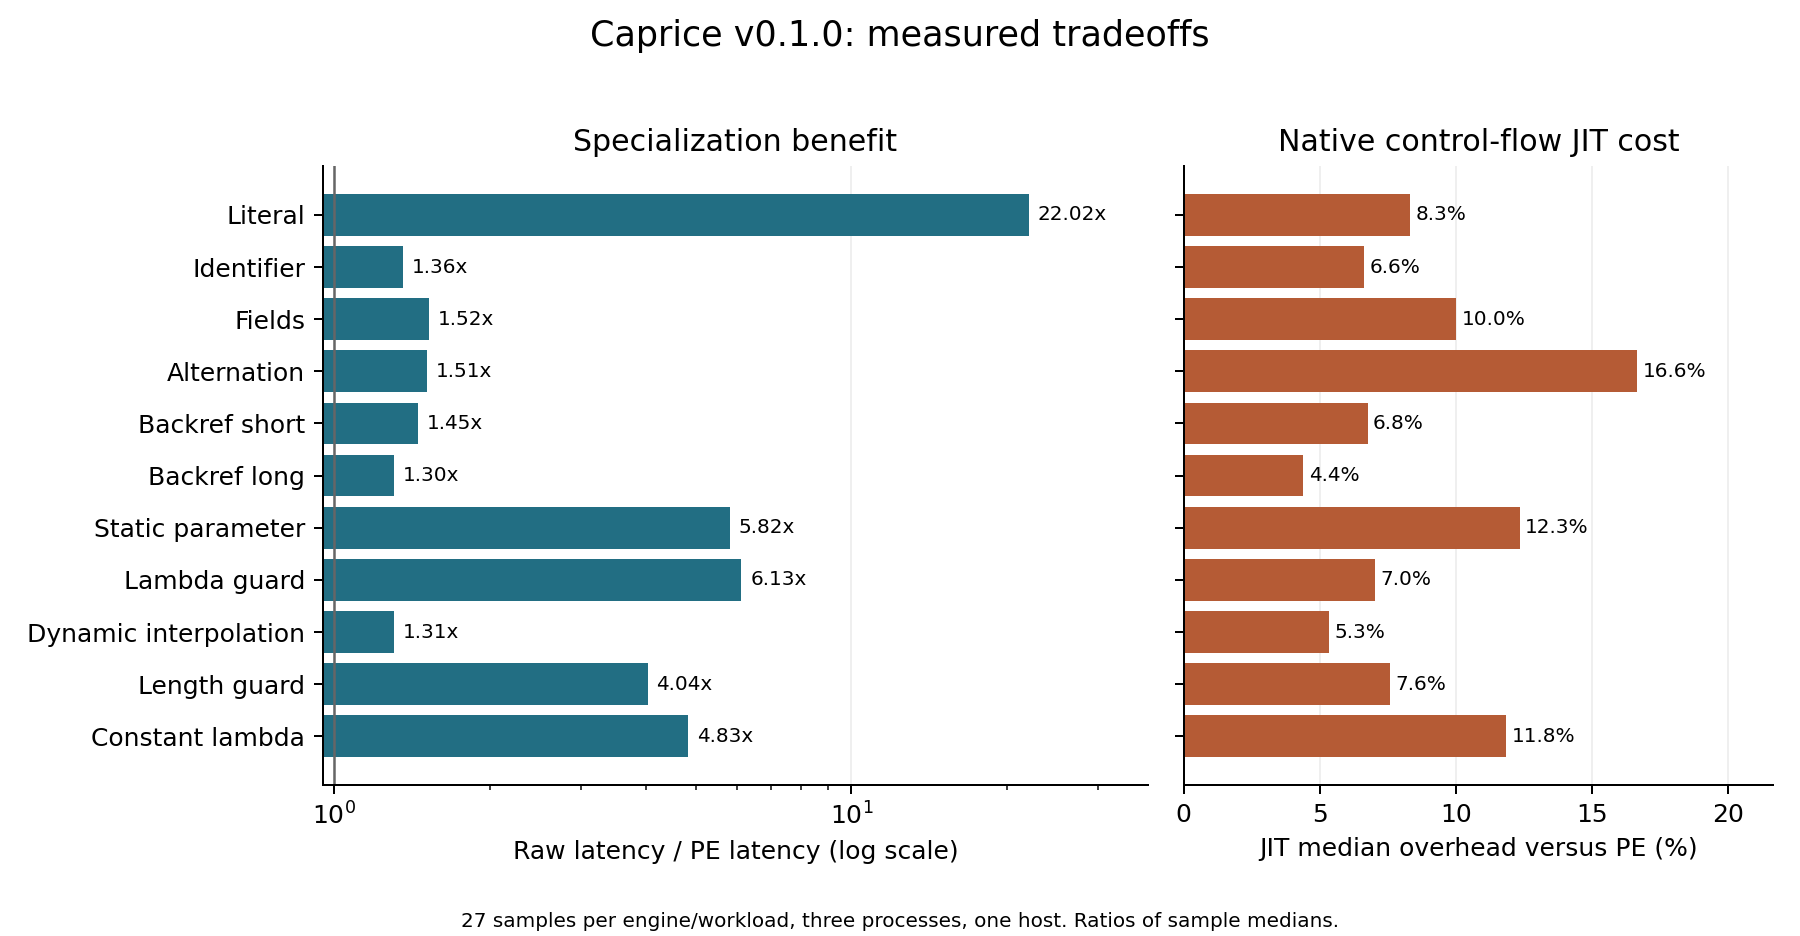
\includegraphics[width=1\textwidth,height=\textheight]{performance.png}
\caption{Ratios of measured medians: specialization improves this
corpus, while the native control-flow JIT adds overhead.}
\end{figure}

\newpage

Median \textbf{microseconds to construct the engine} are shown below,
including parsing and, where selected, PE and JIT compilation. Baseline
construction includes its translated regex but no dynamically compiled
host callback; the small host predicate functions are already compiled
into the benchmark executable.

\begin{longtable}[]{@{}
  >{\raggedright\arraybackslash}p{(\columnwidth - 14\tabcolsep) * \real{0.2727}}
  >{\raggedleft\arraybackslash}p{(\columnwidth - 14\tabcolsep) * \real{0.1039}}
  >{\raggedleft\arraybackslash}p{(\columnwidth - 14\tabcolsep) * \real{0.1039}}
  >{\raggedleft\arraybackslash}p{(\columnwidth - 14\tabcolsep) * \real{0.1039}}
  >{\raggedleft\arraybackslash}p{(\columnwidth - 14\tabcolsep) * \real{0.1039}}
  >{\raggedleft\arraybackslash}p{(\columnwidth - 14\tabcolsep) * \real{0.1039}}
  >{\raggedleft\arraybackslash}p{(\columnwidth - 14\tabcolsep) * \real{0.1039}}
  >{\raggedleft\arraybackslash}p{(\columnwidth - 14\tabcolsep) * \real{0.1039}}@{}}
\toprule\noalign{}
\begin{minipage}[b]{\linewidth}\raggedright
Workload
\end{minipage} & \begin{minipage}[b]{\linewidth}\raggedleft
Raw
\end{minipage} & \begin{minipage}[b]{\linewidth}\raggedleft
PE
\end{minipage} & \begin{minipage}[b]{\linewidth}\raggedleft
JIT
\end{minipage} & \begin{minipage}[b]{\linewidth}\raggedleft
PCRE
\end{minipage} & \begin{minipage}[b]{\linewidth}\raggedleft
PCRE-JIT
\end{minipage} & \begin{minipage}[b]{\linewidth}\raggedleft
Rust
\end{minipage} & \begin{minipage}[b]{\linewidth}\raggedleft
Python
\end{minipage} \\
\midrule\noalign{}
\endhead
\bottomrule\noalign{}
\endlastfoot
Literal & 4.0 & 4.3 & 186.7 & 2.0 & 5.0 & 14.0 & 38.3 \\
Identifier & 1.6 & 0.8 & 265.0 & 0.9 & 4.0 & 28.2 & 30.3 \\
Fields & 0.9 & 1.0 & 338.9 & 0.9 & 5.4 & 11.7 & 30.4 \\
Alternation & 2.1 & 2.9 & 445.9 & 1.4 & 5.2 & 18.8 & 39.1 \\
Backref short & 1.0 & 0.8 & 267.8 & 0.9 & 4.8 & - & 21.8 \\
Backref long & 6.1 & 1.1 & 276.7 & 1.0 & 5.6 & - & 23.3 \\
Static parameter & 1.6 & 1.8 & 266.0 & 1.4 & 4.4 & 14.3 & 30.5 \\
Lambda guard & 2.5 & 2.8 & 293.7 & 0.7 & 3.6 & 9.3 & 19.3 \\
Dynamic interpolation & 1.6 & 1.3 & 273.4 & 1.1 & 5.5 & 24.9 & 29.6 \\
Length guard & 1.4 & 1.6 & 275.0 & 0.7 & 3.5 & 8.7 & 18.6 \\
Constant lambda & 3.3 & 3.8 & 179.0 & 0.5 & 2.8 & 7.0 & 12.6 \\
\end{longtable}

For compile cost \(C\) and repeated match latency \(t\), total cost
after \(N\) uses is \(C+Nt\). Given alternatives \(A\) and \(B\), when
\(C_B>C_A\) and \(t_B<t_A\), the break-even use count satisfies

\[ N>\frac{C_B-C_A}{t_A-t_B}. \]

When \(B\) has both higher compile cost and no lower matching latency,
no positive break-even count follows from those measurements. For JIT
versus PE, the measured median compilation and matching costs are both
higher in all 11 workloads, so no positive break-even count is
demonstrated. This is a property of measured implementations, not a
theorem about all possible partial evaluators or native compilers.

The helper-heavy JIT retains string allocation, capture copying, opcode
dispatch inside helpers, and FFI transitions. Compiling the outer
control-flow graph alone therefore does not guarantee an improvement.
The literal and static-parameter results demonstrate effective
specialization; the dynamic and capture-heavy workloads show the cost of
the remaining runtime. Improvements to native primitive lowering or
persistent capture snapshots require new measurements and proof
obligations.

The raw VM emits one instruction per literal byte. Its largest measured
speedup specifically reflects removing that dispatch overhead; existing
engines already perform their own literal optimizations. The reported PE
effects include the complete specialization pipeline, including
class-repeat fusion and end-check hoisting, rather than isolating
constant folding alone.

An additional adversarial probe uses \texttt{(?:a\textbar{}aa)*b} on
\(a^n\) for \(n\in\{8,12,16,20,24,28\}\). All three Caprice modes reach
the one-million-dispatch budget at lengths 24 and 28 in each process
run; the existing PCRE2 and Rust regex baselines reject without
exhausting that budget or returning an error. This probe is a single
cold decision per process and is reported separately from the warm
benchmark; the regular baseline's startup costs are visible. PCRE2 can
reject this particular family using its required-byte optimization. The
result neither demonstrates that every backtracking engine is vulnerable
on these inputs nor establishes a linear bound for Caprice.

\hypertarget{cost-equivalence-and-limitations}{%
\subsection{10. Cost, equivalence, and
limitations}\label{cost-equivalence-and-limitations}}

Observational equivalence is symmetric; runtime improvement is not.
Attach compilation cost and a workload-indexed latency function to the
directed rewrite presentation before localization. If a rewrite is
reversed after localization, its former compilation cost cannot simply
become a negative time. Hence semantic localization intentionally
forgets some operational information. A correct implementation fiber may
contain both faster and slower realizers.

The formal model uses finite byte strings and pure operators. The Rust
program implements a deliberately small syntax and eager JIT
construction; it has no hotness threshold, persistent code cache, SIMD
lowering, regular-fragment DFA fallback, or proof-carrying machine code.
The Lean proof covers a generic typed expression kernel, not the full
regex semantics. The higher-categorical construction organizes
certificates and observations; it is not evidence that the
implementation computes homotopy types at runtime. The single-host
synthetic evaluation cannot support an across-the-board performance
ranking.

The presheaf and Lean models permit partially supplied static worlds.
The Rust API currently requires every named static parameter at
construction; captured subject data remain dynamic. It does not yet
expose incremental parameter specialization or an
optimization-certificate checker.

The most direct next engineering steps are lowering string comparisons
and capture access into native code, representing repeat alternatives
without cloning all captures, integrating a linear-time backend for a
certified regular fragment, and comparing internal predicates against
PCRE2 callouts. Each must preserve both capture observations and branch
priority. A richer lambda language would need a renewed normalization
and cost argument; adding arbitrary Python or Ruby evaluation would
invalidate the present totality claim.

\hypertarget{reproducibility-and-authorship}{%
\subsection{11. Reproducibility and
authorship}\label{reproducibility-and-authorship}}

The accompanying version 0.1.0 bundle contains Rust source, a locked
dependency graph, CLI examples, corpus generators, per-sample matching
and compilation measurements, stress results, environment metadata, the
Lean source and successful checker output, and the paper in Markdown,
LaTeX, HTML, and PDF. Run \texttt{cargo\ test\ -\/-release\ -\/-locked},
build the release binaries, and execute
\texttt{python3\ scripts/run\_benchmarks.py}. PCRE2 development
libraries are required. The Lean proof checks with
\texttt{lean\ formal/Specialization.lean}. An optional compatibility
shim is documented for hosts that expose \texttt{/proc/self/exe} but not
\texttt{/proc/\textless{}pid\textgreater{}/exe}; it changes
executable-path discovery only and does not modify Lean's kernel.

\textbf{Authorship and automation disclosure.} Submitted by an anonymous
responsible author. An AI assistant assisted with conceptual
formulation, code generation, proofs, testing, benchmarking, and
manuscript preparation. Benchmark numbers are outputs of the included
executions, not model estimates. The anonymous author authorized
submission and accepted the journal's interaction terms. No human peer
review, editorial acceptance, independent replication, or end-to-end
formal verification is claimed.

\hypertarget{references}{%
\subsection{References}\label{references}}

\begin{enumerate}
\def\labelenumi{\arabic{enumi}.}
\tightlist
\item
  N. D. Jones, C. K. Gomard, and P. Sestoft. \emph{Partial Evaluation
  and Automatic Program Generation}. Prentice Hall, 1993.
  Author-maintained text and materials:
  \url{https://raspi.itu.dk/people/sestoft/pebook/pebook.html}.
\item
  M. L. Schmid. \emph{Regular Expressions with Backreferences:
  Polynomial-Time Matching Techniques}. arXiv:1903.05896, revised 2024.
  \url{https://arxiv.org/abs/1903.05896}.
\item
  PCRE2 project. \emph{PCRE2 just-in-time compiler support}.
  \url{https://www.pcre.org/current/doc/html/pcre2jit.html}.
\item
  PCRE2 project. \emph{PCRE2 callout specification}.
  \url{https://www.pcre.org/current/doc/html/pcre2callout.html}.
\item
  Rust regex maintainers. \emph{regex crate documentation}.
  \url{https://docs.rs/regex/1.12.2/regex/}.
\item
  J. Lurie. \emph{Higher Topos Theory}. Annals of Mathematics Studies
  170, Princeton University Press, 2009. Author's text:
  \url{https://www.math.ias.edu/~lurie/papers/HTT.pdf}.
\item
  R. Haugseng. \emph{Iterated Spans and Classical Topological Field
  Theories}. Mathematische Zeitschrift 289 (2018), 1427-1488.
  \url{https://arxiv.org/abs/1409.0837}.
\item
  Bytecode Alliance. \emph{Cranelift JIT demonstration and
  implementation documentation}.
  \url{https://github.com/bytecodealliance/cranelift-jit-demo};
  \url{https://docs.rs/cranelift-jit/0.125.3/cranelift_jit/}.
\item
  Python Software Foundation. \emph{re: Regular expression operations}.
  \url{https://docs.python.org/3/library/re.html}.
\item
  R. Cox. \emph{Regular Expression Matching Can Be Simple and Fast}.
  2007. \url{https://swtch.com/~rsc/regexp/regexp1.html}.
\item
  D. D. Freydenberger and M. L. Schmid. \emph{Deterministic Regular
  Expressions with Back-References}. Journal of Computer and System
  Sciences 105 (2019), 1-39. \url{https://arxiv.org/abs/1802.01508}.
\item
  J. Avigad, L. de Moura, S. Kong, and S. Ullrich. \emph{Theorem Proving
  in Lean 4}. \url{https://lean-lang.org/theorem_proving_in_lean4/}. The
  checked version here is pinned separately to Lean 4.19.0.
\end{enumerate}

All reference URLs were accessed during preparation on October 24, 2026
(America/Los\_Angeles). The cited current documentation may describe
newer releases; the benchmark versions are recorded separately.

\end{document}
